\documentclass[11pt,a4paper]{article}

\usepackage[margin=2.2cm]{geometry}
\usepackage{graphicx}
\usepackage{xcolor}
\usepackage{booktabs}
\usepackage{array}
\usepackage{tabularx}
\usepackage{enumitem}
\usepackage{hyperref}
\usepackage{tikz}
\usetikzlibrary{arrows.meta,positioning,shapes.geometric}

\definecolor{halalgreen}{RGB}{4,120,87}
\definecolor{halallight}{RGB}{236,253,245}
\definecolor{halalamber}{RGB}{180,83,9}
\definecolor{halalred}{RGB}{185,28,28}

\hypersetup{colorlinks=true, linkcolor=halalgreen, urlcolor=halalgreen}

\setlength{\parskip}{0.5em}
\setlength{\parindent}{0pt}

\newcommand{\sectionline}{\vspace{0.3em}\noindent\rule{\textwidth}{0.6pt}\vspace{0.6em}}

\begin{document}

\begin{center}
  {\LARGE\bfseries\color{halalgreen} HalalChain}\\[0.4em]
  {\large A Simple Guide to Our Research and Application}\\[0.8em]
  {\normalsize For reviewers, stakeholders, and non-technical readers}\\[1.2em]
\end{center}

\noindent
\textbf{Authors:} Muhammad Fatih Maulana, Rio Ferdana Sudrajat, Muhammad Rahardian Baihaqi, Muhammad Fahriza Pratama, Yazid Zinky Arisona, Muhammad Fauzan Lubada\\
\textbf{Institution:} Universitas Islam Negeri Sunan Gunung Djati Bandung, Indonesia\\
\textbf{Full paper:} IEEE-format manuscript in \texttt{paper/main.pdf}\\
\textbf{Live demo:} \url{https://web-six-ivory-36.vercel.app/}

\sectionline

\section*{1. Why does this research matter?}

Indonesia requires halal labeling for many food products. Certification involves producers, government bodies (BPJPH), and religious auditors (often through MUI). Despite progress, three trust problems remain:

\begin{enumerate}[leftmargin=1.4em, itemsep=0.35em]
  \item \textbf{Certificates can be copied.} A paper or PDF label does not prove that \emph{this specific production batch} was actually audited.
  \item \textbf{Central databases can be changed.} If one administrator controls the records, outsiders cannot independently verify whether history was altered.
  \item \textbf{Existing digital systems are often too expensive.} Large enterprise blockchain platforms assume big companies with IT teams and complex wallets---not typical UMKM (micro and small) food producers.
\end{enumerate}

\noindent
\textbf{HalalChain} is our answer: a simple, open system that ties each product \textbf{batch} to a permanent, public audit record---while letting ordinary consumers check status with a phone, \textbf{without installing a crypto wallet}.

\sectionline

\section*{2. What is HalalChain in one sentence?}

HalalChain is a \textbf{batch traceability system} where:
\begin{itemize}[leftmargin=1.4em, itemsep=0.25em]
  \item producers register a batch and upload supporting documents,
  \item accredited auditors approve or reject that batch on a public digital ledger,
  \item consumers scan a QR code and instantly see whether that batch is certified, pending, rejected, or revoked.
\end{itemize}

\noindent
Think of it as a \textbf{transparent audit log} for halal batches---not a replacement for official halal law or religious rulings.

\sectionline

\section*{3. How does the system work? (Plain-language flow)}

\begin{center}
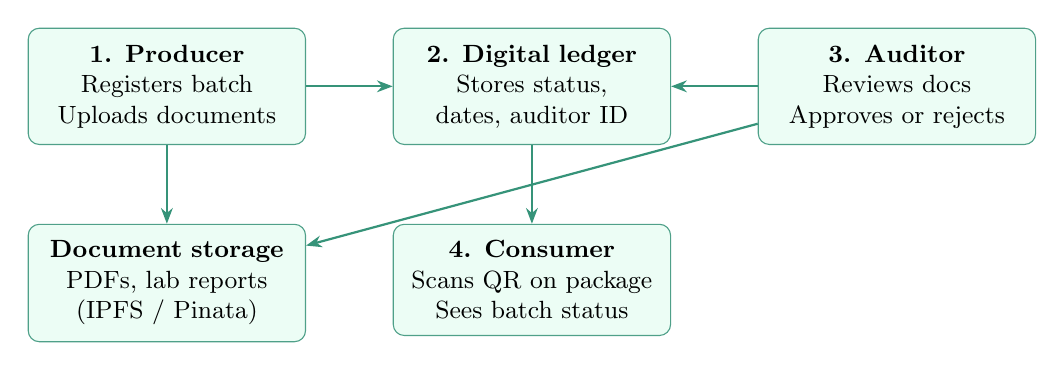
\begin{tikzpicture}[
  node distance=0.55cm and 0.4cm,
  box/.style={draw=halalgreen!70, fill=halallight, rounded corners=4pt,
    align=center, font=\small, inner sep=6pt, text width=3.1cm},
  arr/.style={-{Stealth[length=2mm]}, thick, halalgreen!80}
]
  \node[box] (prod) {\textbf{1. Producer}\\Registers batch\\Uploads documents};
  \node[box, right=1.1cm of prod] (chain) {\textbf{2. Digital ledger}\\Stores status,\\dates, auditor ID};
  \node[box, right=1.1cm of chain] (aud) {\textbf{3. Auditor}\\Reviews docs\\Approves or rejects};
  \node[box, below=1.0cm of chain] (cons) {\textbf{4. Consumer}\\Scans QR on package\\Sees batch status};
  \node[box, below=1.0cm of prod] (ipfs) {\textbf{Document storage}\\PDFs, lab reports\\(IPFS / Pinata)};

  \draw[arr] (prod) -- (chain);
  \draw[arr] (aud) -- (chain);
  \draw[arr] (chain) -- (cons);
  \draw[arr] (prod) -- (ipfs);
  \draw[arr] (aud) -- (ipfs);
\end{tikzpicture}
\end{center}

\vspace{0.4em}
\noindent
\textbf{What goes where?}
\begin{itemize}[leftmargin=1.4em, itemsep=0.2em]
  \item \textbf{On the ledger (small, permanent):} batch status, who registered it, who audited it, when, document references, rejection reasons.
  \item \textbf{Off the ledger (large files):} ingredient lists, process photos, lab reports, audit attachments---stored on IPFS (a distributed file network) and linked by a secure reference (CID).
\end{itemize}

\noindent
This split keeps costs low while preserving a tamper-evident record of \emph{who decided what, and when}.

\sectionline

\section*{4. The three user roles in the web application}

\begin{tabularx}{\textwidth}{@{}>{\raggedright\arraybackslash}p{2.1cm}X@{}}
\toprule
\textbf{Role} & \textbf{What they do in the app} \\
\midrule
\textbf{Producer} & Registers a new product batch, uploads supporting files, receives a batch number and QR code for packaging. Cannot self-certify as halal. \\
\textbf{Auditor} & Sees pending batches, opens documents, then marks a batch as \emph{Verified}, \emph{Rejected}, or (if needed) \emph{Revoked}. Actions are permanently recorded. \\
\textbf{Consumer} & Opens a verify link or scans a QR code. Reads the status page only---no account, no wallet, no cryptocurrency needed. \\
\bottomrule
\end{tabularx}

\vspace{0.5em}
\noindent
\textbf{Batch statuses shown to consumers:}
\begin{itemize}[leftmargin=1.4em, itemsep=0.15em]
  \item \textcolor{halalgreen}{\textbf{Verified}} --- ``Tersertifikasi Halal'' / Halal Certified
  \item \textcolor{halalamber}{\textbf{Pending}} --- waiting for auditor review
  \item \textcolor{halalred}{\textbf{Rejected}} --- not certified; reason is shown
  \item \textbf{Revoked} --- was certified before, but later withdrawn
\end{itemize}

\sectionline

\section*{5. Important design rule: rejection cannot be secretly undone}

If an auditor \textbf{rejects} a batch, that same batch ID can \textbf{never} be upgraded to ``verified'' later. This is enforced by the smart contract, not by policy alone.

If a producer fixes problems, they submit a \textbf{new revision batch} linked to the old rejected one. Consumers can still inspect the original rejection and the new approved batch---supporting transparency and accountability (\emph{Amanah}).

\sectionline

\section*{6. Islamic ethical principles in engineering terms}

Our paper maps widely cited Islamic values to concrete system behavior. This is \textbf{engineering design}, not a religious fatwa.

\begin{tabularx}{\textwidth}{@{}>{\raggedright\arraybackslash}p{2.3cm}>{\raggedright\arraybackslash}p{3.2cm}X@{}}
\toprule
\textbf{Principle} & \textbf{Meaning} & \textbf{How HalalChain implements it} \\
\midrule
Amanah & Trustworthiness & Audit outcomes cannot be silently rewritten; rejections stay on record. \\
Thoyyib & Wholesomeness & The consumer page shows a positive halal result only for verified batches. \\
Adl & Justice / fairness & Anyone can read batch status from the public ledger; no private gatekeeper API. \\
Hisba & Accountability & Every approval records \emph{which auditor address} acted and \emph{when}. \\
\bottomrule
\end{tabularx}

\sectionline

\section*{7. What did we build and test?}

\textbf{Software delivered:}
\begin{itemize}[leftmargin=1.4em, itemsep=0.2em]
  \item Smart contract (\texttt{HalalChain.sol}) with role-based access control
  \item Producer, auditor, and consumer web dashboards (Next.js)
  \item Open-source repository: \url{https://github.com/Fatihmaull/halal-chain}
\end{itemize}

\textbf{Evaluation (Ethereum Sepolia testnet, June 2026):}
\begin{itemize}[leftmargin=1.4em, itemsep=0.2em]
  \item \textbf{Scenario A:} Batch registered and verified $\rightarrow$ consumer page shows certified status
  \item \textbf{Scenario B:} Batch rejected, then resubmitted as revision $\rightarrow$ new batch verified with link to parent
  \item \textbf{Scenario C:} Attempt to approve a rejected batch fails $\rightarrow$ tamper resistance confirmed
  \item \textbf{Cost signal:} Registering a batch and verifying it cost fractions of a cent in test ETH; reading status for consumers costs nothing
\end{itemize}

\sectionline

\section*{8. Try the live prototype}

\begin{tabularx}{\textwidth}{@{}lX@{}}
\toprule
\textbf{Page} & \textbf{URL} \\
\midrule
Home & \url{https://web-six-ivory-36.vercel.app/} \\
Verified example (Batch \#1) & \url{https://web-six-ivory-36.vercel.app/verify/1} \\
Rejected example (Batch \#2) & \url{https://web-six-ivory-36.vercel.app/verify/2} \\
Revision example (Batch \#3) & \url{https://web-six-ivory-36.vercel.app/verify/3} \\
On-chain contract & \url{https://sepolia.etherscan.io/address/0xDaCA688e86F438A7cD6B0C9B69606C67CE85Dc92} \\
\bottomrule
\end{tabularx}

\sectionline

\section*{9. What HalalChain is \emph{not}}

\begin{itemize}[leftmargin=1.4em, itemsep=0.25em]
  \item It does \textbf{not} replace BPJPH, MUI, or official halal certification law.
  \item It does \textbf{not} automatically analyze ingredients or slaughter methods.
  \item It does \textbf{not} prove halal compliance by itself---it proves \textbf{which auditor approved which documents at which time}, on a record that is hard to alter retroactively.
\end{itemize}

\sectionline

\section*{10. Research questions addressed}

\begin{enumerate}[leftmargin=1.4em, itemsep=0.3em]
  \item Can a \textbf{minimal} blockchain design give UMKM-affordable, immutable batch verification?
  \item How should we split data between the ledger (status) and file storage (documents) for cost and trust?
  \item Can Islamic ethical requirements be translated into \textbf{testable} software properties without confusing engineering with religious judgment?
\end{enumerate}

\vspace{0.8em}
\noindent
\textbf{For the full technical treatment}---architecture, contract specification, gas tables, limitations, and bibliography---please see the complete paper in \texttt{paper/main.pdf}.

\vfill
\begin{center}
\small
\textcolor{gray}{HalalChain Overview --- UIN Sunan Gunung Djati Bandung --- \today}
\end{center}

\end{document}
